
%% bare_conf_compsoc.tex
%% V1.4b
%% 2015/08/26
%% by Michael Shell
%% See:
%% http://www.michaelshell.org/
%% for current contact information.
%%
%% This is a skeleton file demonstrating the use of IEEEtran.cls
%% (requires IEEEtran.cls version 1.8b or later) with an IEEE Computer
%% Society conference paper.
%%
%% Support sites:
%% http://www.michaelshell.org/tex/ieeetran/
%% http://www.ctan.org/pkg/ieeetran
%% and
%% http://www.ieee.org/

%%*************************************************************************
%% Legal Notice:
%% This code is offered as-is without any warranty either expressed or
%% implied; without even the implied warranty of MERCHANTABILITY or
%% FITNESS FOR A PARTICULAR PURPOSE! 
%% User assumes all risk.
%% In no event shall the IEEE or any contributor to this code be liable for
%% any damages or losses, including, but not limited to, incidental,
%% consequential, or any other damages, resulting from the use or misuse
%% of any information contained here.
%%
%% All comments are the opinions of their respective authors and are not
%% necessarily endorsed by the IEEE.
%%
%% This work is distributed under the LaTeX Project Public License (LPPL)
%% ( http://www.latex-project.org/ ) version 1.3, and may be freely used,
%% distributed and modified. A copy of the LPPL, version 1.3, is included
%% in the base LaTeX documentation of all distributions of LaTeX released
%% 2003/12/01 or later.
%% Retain all contribution notices and credits.
%% ** Modified files should be clearly indicated as such, including  **
%% ** renaming them and changing author support contact information. **
%%*************************************************************************


% *** Authors should verify (and, if needed, correct) their LaTeX system  ***
% *** with the testflow diagnostic prior to trusting their LaTeX platform ***
% *** with production work. The IEEE's font choices and paper sizes can   ***
% *** trigger bugs that do not appear when using other class files.       ***                          ***
% The testflow support page is at:
% http://www.michaelshell.org/tex/testflow/



\documentclass[conference,compsoc]{IEEEtran}
% Some/most Computer Society conferences require the compsoc mode option,
% but others may want the standard conference format.
%
% If IEEEtran.cls has not been installed into the LaTeX system files,
% manually specify the path to it like:
% \documentclass[conference,compsoc]{../sty/IEEEtran}





% Some very useful LaTeX packages include:
% (uncomment the ones you want to load)


% *** MISC UTILITY PACKAGES ***
%
%\usepackage{ifpdf}
% Heiko Oberdiek's ifpdf.sty is very useful if you need conditional
% compilation based on whether the output is pdf or dvi.
% usage:
% \ifpdf
%   % pdf code
% \else
%   % dvi code
% \fi
% The latest version of ifpdf.sty can be obtained from:
% http://www.ctan.org/pkg/ifpdf
% Also, note that IEEEtran.cls V1.7 and later provides a builtin
% \ifCLASSINFOpdf conditional that works the same way.
% When switching from latex to pdflatex and vice-versa, the compiler may
% have to be run twice to clear warning/error messages.






% *** CITATION PACKAGES ***
%
\ifCLASSOPTIONcompsoc
  % IEEE Computer Society needs nocompress option
  % requires cite.sty v4.0 or later (November 2003)
  \usepackage[nocompress]{cite}
\else
  % normal IEEE
  \usepackage{cite}
\fi
% cite.sty was written by Donald Arseneau
% V1.6 and later of IEEEtran pre-defines the format of the cite.sty package
% \cite{} output to follow that of the IEEE. Loading the cite package will
% result in citation numbers being automatically sorted and properly
% "compressed/ranged". e.g., [1], [9], [2], [7], [5], [6] without using
% cite.sty will become [1], [2], [5]--[7], [9] using cite.sty. cite.sty's
% \cite will automatically add leading space, if needed. Use cite.sty's
% noadjust option (cite.sty V3.8 and later) if you want to turn this off
% such as if a citation ever needs to be enclosed in parenthesis.
% cite.sty is already installed on most LaTeX systems. Be sure and use
% version 5.0 (2009-03-20) and later if using hyperref.sty.
% The latest version can be obtained at:
% http://www.ctan.org/pkg/cite
% The documentation is contained in the cite.sty file itself.
%
% Note that some packages require special options to format as the Computer
% Society requires. In particular, Computer Society  papers do not use
% compressed citation ranges as is done in typical IEEE papers
% (e.g., [1]-[4]). Instead, they list every citation separately in order
% (e.g., [1], [2], [3], [4]). To get the latter we need to load the cite
% package with the nocompress option which is supported by cite.sty v4.0
% and later.





% *** GRAPHICS RELATED PACKAGES ***
%
\ifCLASSINFOpdf
  % \usepackage[pdftex]{graphicx}
  % declare the path(s) where your graphic files are
  % \graphicspath{{../pdf/}{../jpeg/}}
  % and their extensions so you won't have to specify these with
  % every instance of \includegraphics
  % \DeclareGraphicsExtensions{.pdf,.jpeg,.png}
\else
  % or other class option (dvipsone, dvipdf, if not using dvips). graphicx
  % will default to the driver specified in the system graphics.cfg if no
  % driver is specified.
  % \usepackage[dvips]{graphicx}
  % declare the path(s) where your graphic files are
  % \graphicspath{{../eps/}}
  % and their extensions so you won't have to specify these with
  % every instance of \includegraphics
  % \DeclareGraphicsExtensions{.eps}
\fi
% graphicx was written by David Carlisle and Sebastian Rahtz. It is
% required if you want graphics, photos, etc. graphicx.sty is already
% installed on most LaTeX systems. The latest version and documentation
% can be obtained at: 
% http://www.ctan.org/pkg/graphicx
% Another good source of documentation is "Using Imported Graphics in
% LaTeX2e" by Keith Reckdahl which can be found at:
% http://www.ctan.org/pkg/epslatex
%
% latex, and pdflatex in dvi mode, support graphics in encapsulated
% postscript (.eps) format. pdflatex in pdf mode supports graphics
% in .pdf, .jpeg, .png and .mps (metapost) formats. Users should ensure
% that all non-photo figures use a vector format (.eps, .pdf, .mps) and
% not a bitmapped formats (.jpeg, .png). The IEEE frowns on bitmapped formats
% which can result in "jaggedy"/blurry rendering of lines and letters as
% well as large increases in file sizes.
%
% You can find documentation about the pdfTeX application at:
% http://www.tug.org/applications/pdftex





% *** MATH PACKAGES ***
%
\usepackage{amsmath}
% A popular package from the American Mathematical Society that provides
% many useful and powerful commands for dealing with mathematics.
%
% Note that the amsmath package sets \interdisplaylinepenalty to 10000
% thus preventing page breaks from occurring within multiline equations. Use:
%\interdisplaylinepenalty=2500
% after loading amsmath to restore such page breaks as IEEEtran.cls normally
% does. amsmath.sty is already installed on most LaTeX systems. The latest
% version and documentation can be obtained at:
% http://www.ctan.org/pkg/amsmath





% *** SPECIALIZED LIST PACKAGES ***
%
%\usepackage{algorithmic}
% algorithmic.sty was written by Peter Williams and Rogerio Brito.
% This package provides an algorithmic environment fo describing algorithms.
% You can use the algorithmic environment in-text or within a figure
% environment to provide for a floating algorithm. Do NOT use the algorithm
% floating environment provided by algorithm.sty (by the same authors) or
% algorithm2e.sty (by Christophe Fiorio) as the IEEE does not use dedicated
% algorithm float types and packages that provide these will not provide
% correct IEEE style captions. The latest version and documentation of
% algorithmic.sty can be obtained at:
% http://www.ctan.org/pkg/algorithms
% Also of interest may be the (relatively newer and more customizable)
% algorithmicx.sty package by Szasz Janos:
% http://www.ctan.org/pkg/algorithmicx




% *** ALIGNMENT PACKAGES ***
%
%\usepackage{array}
% Frank Mittelbach's and David Carlisle's array.sty patches and improves
% the standard LaTeX2e array and tabular environments to provide better
% appearance and additional user controls. As the default LaTeX2e table
% generation code is lacking to the point of almost being broken with
% respect to the quality of the end results, all users are strongly
% advised to use an enhanced (at the very least that provided by array.sty)
% set of table tools. array.sty is already installed on most systems. The
% latest version and documentation can be obtained at:
% http://www.ctan.org/pkg/array


% IEEEtran contains the IEEEeqnarray family of commands that can be used to
% generate multiline equations as well as matrices, tables, etc., of high
% quality.


%% Implement below code to enable code listing within the doc
\usepackage{listings}
\usepackage{color}

\usepackage{algorithm,algorithmic}
\usepackage{xcolor}


\definecolor{dkgreen}{rgb}{0,0.6,0}
\definecolor{gray}{rgb}{0.5,0.5,0.5}
\definecolor{mauve}{rgb}{0.58,0,0.82}

\lstset{frame=tb,
  language=C++,
  aboveskip=3mm,
  belowskip=3mm,
  showstringspaces=false,
  columns=flexible,
  basicstyle={\small\ttfamily},
  numbers=none,
  numberstyle=\tiny\color{gray},
  keywordstyle=\color{blue},
  commentstyle=\color{dkgreen},
  stringstyle=\color{mauve},
  breaklines=true,
  breakatwhitespace=true,
  tabsize=4
}

\usepackage{graphicx}
\usepackage{subcaption}


% *** SUBFIGURE PACKAGES ***
%\ifCLASSOPTIONcompsoc
%  \usepackage[caption=false,font=footnotesize,labelfont=sf,textfont=sf]{subfig}
%\else
%  \usepackage[caption=false,font=footnotesize]{subfig}
%\fi
% subfig.sty, written by Steven Douglas Cochran, is the modern replacement
% for subfigure.sty, the latter of which is no longer maintained and is
% incompatible with some LaTeX packages including fixltx2e. However,
% subfig.sty requires and automatically loads Axel Sommerfeldt's caption.sty
% which will override IEEEtran.cls' handling of captions and this will result
% in non-IEEE style figure/table captions. To prevent this problem, be sure
% and invoke subfig.sty's "caption=false" package option (available since
% subfig.sty version 1.3, 2005/06/28) as this is will preserve IEEEtran.cls
% handling of captions.
% Note that the Computer Society format requires a sans serif font rather
% than the serif font used in traditional IEEE formatting and thus the need
% to invoke different subfig.sty package options depending on whether
% compsoc mode has been enabled.
%
% The latest version and documentation of subfig.sty can be obtained at:
% http://www.ctan.org/pkg/subfig




% *** FLOAT PACKAGES ***
%
%\usepackage{fixltx2e}
% fixltx2e, the successor to the earlier fix2col.sty, was written by
% Frank Mittelbach and David Carlisle. This package corrects a few problems
% in the LaTeX2e kernel, the most notable of which is that in current
% LaTeX2e releases, the ordering of single and double column floats is not
% guaranteed to be preserved. Thus, an unpatched LaTeX2e can allow a
% single column figure to be placed prior to an earlier double column
% figure.
% Be aware that LaTeX2e kernels dated 2015 and later have fixltx2e.sty's
% corrections already built into the system in which case a warning will
% be issued if an attempt is made to load fixltx2e.sty as it is no longer
% needed.
% The latest version and documentation can be found at:
% http://www.ctan.org/pkg/fixltx2e


%\usepackage{stfloats}
% stfloats.sty was written by Sigitas Tolusis. This package gives LaTeX2e
% the ability to do double column floats at the bottom of the page as well
% as the top. (e.g., "\begin{figure*}[!b]" is not normally possible in
% LaTeX2e). It also provides a command:
%\fnbelowfloat
% to enable the placement of footnotes below bottom floats (the standard
% LaTeX2e kernel puts them above bottom floats). This is an invasive package
% which rewrites many portions of the LaTeX2e float routines. It may not work
% with other packages that modify the LaTeX2e float routines. The latest
% version and documentation can be obtained at:
% http://www.ctan.org/pkg/stfloats
% Do not use the stfloats baselinefloat ability as the IEEE does not allow
% \baselineskip to stretch. Authors submitting work to the IEEE should note
% that the IEEE rarely uses double column equations and that authors should try
% to avoid such use. Do not be tempted to use the cuted.sty or midfloat.sty
% packages (also by Sigitas Tolusis) as the IEEE does not format its papers in
% such ways.
% Do not attempt to use stfloats with fixltx2e as they are incompatible.
% Instead, use Morten Hogholm'a dblfloatfix which combines the features
% of both fixltx2e and stfloats:
%
% \usepackage{dblfloatfix}
% The latest version can be found at:
% http://www.ctan.org/pkg/dblfloatfix




% *** PDF, URL AND HYPERLINK PACKAGES ***
%
%\usepackage{url}
% url.sty was written by Donald Arseneau. It provides better support for
% handling and breaking URLs. url.sty is already installed on most LaTeX
% systems. The latest version and documentation can be obtained at:
% http://www.ctan.org/pkg/url
% Basically, \url{my_url_here}.




% *** Do not adjust lengths that control margins, column widths, etc. ***
% *** Do not use packages that alter fonts (such as pslatex).         ***
% There should be no need to do such things with IEEEtran.cls V1.6 and later.
% (Unless specifically asked to do so by the journal or conference you plan
% to submit to, of course. )


% correct bad hyphenation here
\hyphenation{op-tical net-works semi-conduc-tor}


\begin{document}
%
% paper title
% Titles are generally capitalized except for words such as a, an, and, as,
% at, but, by, for, in, nor, of, on, or, the, to and up, which are usually
% not capitalized unless they are the first or last word of the title.
% Linebreaks \\ can be used within to get better formatting as desired.
% Do not put math or special symbols in the title.
\title{AllScale toolchain pilot application: Development of an advanced data assimilation framework within a parallel computing environment}


% author names and affiliations
% use a multiple column layout for up to three different
% affiliations
\author{\IEEEauthorblockN{Albert Akhriev}
\IEEEauthorblockA{IBM Research - Ireland\\
Email: albert\_akhriev@ie.ibm.com}
\and
\IEEEauthorblockN{Emanuele Ragnoli}
\IEEEauthorblockA{IBM Research - Ireland\\
Email: eragnoli@ie.ibm.com}
\and
\IEEEauthorblockN{Fearghal O'Donncha}
\IEEEauthorblockA{IBM Research - Ireland\\
Email: feardonn@ie.ibm.com}
}
% conference papers do not typically use \thanks and this command
% is locked out in conference mode. If really needed, such as for
% the acknowledgment of grants, issue a \IEEEoverridecommandlockouts
% after \documentclass

% for over three affiliations, or if they all won't fit within the width
% of the page (and note that there is less available width in this regard for
% compsoc conferences compared to traditional conferences), use this
% alternative format:
% 
%\author{\IEEEauthorblockN{Michael Shell\IEEEauthorrefmark{1},
%Homer Simpson\IEEEauthorrefmark{2},
%James Kirk\IEEEauthorrefmark{3}, 
%Montgomery Scott\IEEEauthorrefmark{3} and
%Eldon Tyrell\IEEEauthorrefmark{4}}
%\IEEEauthorblockA{\IEEEauthorrefmark{1}School of Electrical and Computer Engineering\\
%Georgia Institute of Technology,
%Atlanta, Georgia 30332--0250\\ Email: see http://www.michaelshell.org/contact.html}
%\IEEEauthorblockA{\IEEEauthorrefmark{2}Twentieth Century Fox, Springfield, USA\\
%Email: homer@thesimpsons.com}
%\IEEEauthorblockA{\IEEEauthorrefmark{3}Starfleet Academy, San Francisco, California 96678-2391\\
%Telephone: (800) 555--1212, Fax: (888) 555--1212}
%\IEEEauthorblockA{\IEEEauthorrefmark{4}Tyrell Inc., 123 Replicant Street, Los Angeles, California 90210--4321}}




% use for special paper notices
%\IEEEspecialpapernotice{(Invited Paper)}




% make the title area
\maketitle

% As a general rule, do not put math, special symbols or citations
% in the abstract
\begin{abstract}
This paper presents an implementation of a complex PDE based model within a novel programming environment – AllScale. The AllScale toolchain aims to greatly simplify application development in the ExaScale era by siloing development responsibilities. The front-end API provides the developer with a simple C++ development environment and a suite of parallel constructs that denote tasks to be operated concurrently. Lower level tasks related to the machine and system level are managed by computer scientists at the core-level. We present the development of a data assimilation framework for the simulation of advection-diffusion transports within this API. Mathematical formulations and implementations are presented and we evaluate parallel constructs developed within the AllScale User API. The performance of the model from the perspective of both parallel scalability and more importantly ease of development and maintainability are assessed. We demonstrate how the AllScale API can drastically improve developer productivity while maintaining parallel performance. Taking a complex data assimilation model as a use case, we provide a development framework and evaluation test study for the AllScale API.
\end{abstract}

% no keywords




% For peer review papers, you can put extra information on the cover
% page as needed:
% \ifCLASSOPTIONpeerreview
% \begin{center} \bfseries EDICS Category: 3-BBND \end{center}
% \fi
%
% For peerreview papers, this IEEEtran command inserts a page break and
% creates the second title. It will be ignored for other modes.
\IEEEpeerreviewmaketitle


\section{Introduction}

Feasible and scalable systems for the accurate estimation of advection diffusion processes are required in several applications. Examples include forecasting oil spill evolution for remediation efforts~\cite{guo2009modeling}, quantifying the transport of nutrients around aquaculture installations~\cite{odonncha2013physical} and monitoring releases from industrial operations~\cite{koziy1998three}.  Typically, these are provided from the solution of a set of Partial Differential Equations (PDEs) on a discretised grid. To improve the accuracy of the prediction, methods exist to update the solution using measurements of the actual state via data assimilation (DA). DA improves the accuracy of forecasts provided by physical models and evaluates their reliability by optimally combining \emph{a priori} knowledge encoded in equations of mathematical physics with \emph{a posteriori} information in the form of sensor data. 

A key challenge facing the feasible merging of mathematical models and data is computational expense. With the drive to model more realistic and detailed simulations, the computational demands of numerical solutions increase. At the same time, the last few years have seen an increased abundance and availability of sensors data, ranging from satellite data to in-situ marine data. Developing computationally efficient DA implementation is challenging with PDEs since the computational costs and demands escalate with the increase in the degrees of freedom of the corresponding discretization. For this reason, methods that enable practical state estimation approaches by reducing the dimensionality of the problem and distributing across compute resources are very active research areas. 

Domain Decomposition (DD) is a standard tool in many scientific domains to reduce the complexity or computational cost of solution. Some of the factors which have motivated DD approaches include: 1) the solution of the subproblems is qualitatively or quantitatively easier than the original, 2) the original problem does not fit into the available memory space and 3) the subproblems can be solved with some concurrency (i.e. in parallel).

This has facilitated many advances in simulation capabilities in the geosciences with most operational large-scale models adopting this paradigm \cite{michalakes2001development, hu2013scalable, hammond2014evaluating}. In this approach, subdomains are distributed across computational cores and solved independently with a periodic synchronization step to ensure the fidelity of the solution. Synchronization typically occurs at the end of each computational timestep and involves a communication of boundary solution state to neighbour subdomains with MPI being the most popular protocol for exchanging data and synchronizing solutions. To improve computational performance, fine-grained parallelism is often implemented within subdomains, via for-example the OpenMP paradigm.

Synchronization requirements and multiple parallelisation schemas enforced by performance considerations means that the development of efficient code places very high skill demands on the application developer, encompassing knowledge of sophisticated domain related algorithmic formulation and solvers together with complex software engineering skills. This is accentuated as degree of parallelism becomes larger and codes are deployed on hundreds of thousands to millions of computational cores. Indeed, recent efforts have addressed this such as the LFric research project from the UK Met Office that aims to develop a replacement for the Met Office Unified Model in order to meet the challenges which will be presented by the next generation of ExaScale supercomputers \cite{melvin2017lfric}. Design of the model revolves around a principle of a 'separation of concerns', whereby the natural science aspects of the code can be developed without worrying about the underlying architecture, while machine dependent optimisations can be carried out at a high level (by HPC experts).

In this paper we present the paralellisation of a DA scheme for advection-diffusion flows using a novel toolchain that empowers effective development of highly scalable parallel applications. The design of the ExaScale development environment, named the AllScale tool chain, is based on 3 key principles
\begin{enumerate}
\item Enabling the separation of responsibilities in the development of HPC applications,
\item Utilizing industry standard programming languages and preserving compatibility to existing development and debugging tools, as well as,
\item Employing advanced programming language, compilation and runtime system technology to transparently integrate sophisticated services into parallel applications.
\end{enumerate} 
From the application developer perspective, it promises highly increased productivity by hiding all parallel constructs and providing a development API reminiscent of serial applications.

We leverage the AllScale API and toolchain to develop a highly scalable code for the simulation of marine oil spills that combines an advection diffusion model with data assimilation algorithms. The approach combines DA with domain decomposition to 1) reduce the computational expense of DA and 2) facilitate nested recursive parallelism applied to a DA problem by localising state updates to individual subdomains. 
In this study, the global domain is split into subdomains and the equations are discretised on each subdomain. Interface boundary conditions are enforced using a ghost cell approach that overlaps neighbouring solutions. The data assimilation algorithm aligns with the data decomposition strategy by adopting a set of localised data filters unique to each subdomain. The solution is implemented using the novel AllScale API (based on C++ template-style programming) that manages distribution across cores, load balancing and synchronization of solution between subdomains. 

In the remainder of this paper, Section \ref{sec:API} describes the AllScale User API while Section \ref{sec:AMDADOS} details the application governing equations and numerical algorithms. Section \ref{sec:porting} outlines the development of the application within the API and compares with an MPI implementation to provide a qualitative evaluation of impact on developer productivity; performance results and parallel scalability are also presented. Finally, we draw conclusions from the study and present the future research steps.

\section{AllScale API description}
\label{sec:API}
The AllScale API is the facade of the AllScale Environment towards end-user applications. It provides the necessary primitives to express parallelism, data dependencies, and needed synchronization steps within application code. The
API is subdivided into two layers:
\begin{itemize}
\item The AllScale Core API
\item The AllScale User API
\end{itemize}
The Core API provides a concise set of basic generic primitives, comprising
parallel control flow, synchronization, and communication constructs. The User
API is harnessing the expressive power of the Core API to provide specialized
primitives for particular use cases, including basic constructs like parallel loops
as well as more sophisticated functionality offering efficient implementations of
e.g. stencil operations.
The purpose of the subdivision into a Core and User API is to enable the
implementation of a variety of parallel primitives on top of a small, concise set of
central constructs which can be utilized to provide portability among different
implementations of the AllScale Core API.

Thus, the overall task of
providing efficient parallel codes is distributed among three contributors:
\begin{itemize}
\item \textit{the domain expert} aiming on obtaining the most effective algorithmic solution for the problem of interest
\item \textit{the high performance computing expert} able to develop efficient domain specific primitives to be utilized by the domain expert, focusing on e.g. communication and synchronization overheads and cache efficiency
\item \textit{the system level expert} focusing on providing the most flexible and portable implementation of the Core API, thereby handling load management, scheduling, resilience, and hardware management obligations
\end{itemize}

The separation of responsibilities also affects the code base. By shielding the
domain expert from all the underlying details (synchronization, communication,
cache efficiency, scheduling, utilization of low-level parallel APIs ...), the
resulting application code remains free of the otherwise necessary management
code. This positively affects the maintainability of the resulting applications and
thus the productivity of the domain expert.

\subsection{AllScale Core API}
The AllScale Core API provides a concise set of generic primitives for expressing
parallel control flows, communication, and synchronization operations. A detailed description of the AllScale Core API is provided in \cite{allscale_architecure_2017} and is briefly summarised here.

Provision of parallel task control and synchronization is a key component of the API.
The AllScale Core API provides a single primitive for running concurrent tasks.
This primitive, the \textit{prec} operator, is a higher order function combining three
given functions into a new, recursive function. The three combined input
functions are:
\begin{itemize}
\item a function testing for the base case of a recursion
\item a function processing the base case of a recursion
\item a function processing the recursive step case
\end{itemize}
The \textit{prec} operator combines those functions into a new recursive function which,
for a given input parameter, conducts the specified computation accordingly.
Thereby sub-tasks invoked by the step case function may be processed in
parallel.


Similar for parallel constructs, data structures require specification by a uniform set of primitives to be managed by an underlying runtime system. 
To this end, the data structure primitives offered by the core are a mere
specification of any potential type's interfaces and behaviours -- in C++ terms a
concept. Any type, T, to be managed by an AllScale API implementation has to
provide the following properties:

type T has to specify the following types:
\begin{itemize}
\item a type F for fragments of the data storage
\item a type R for addressing sub-ranges of the data structure
 \end{itemize}

Each of those types has to provide operators for pertinent actions such as \textit{create}, \textit{delete}, \textit{resize}, etc.

Finally a key requirement of any application is I/O which is again enabled by the core API. AllScale Core API provides basic primitives
to facilitate high-performance IO while keeping actual implementations abstract.
There are two different kind of IO operations supported:
\begin{itemize}
\item Streaming, supported through an AllScale IO interface facilitating e.g. the writing of simulation results to output streams
\item Memory mapped IO for the structured loading of static input data for which efficient random access operations are required
\end{itemize}

Further details on the AllScale core API are provided in \cite{allscale_architecure_2017}.

\subsection{AllScale user API}

The generic nature of the Core API exceeds the complexity which could be
effectively handled by domain experts for implementing parallel algorithms.
Thus, it is the objective of the AllScale User API layer to provide a set of more
user-friendly constructs for the composition of parallel applications.

The list of constructs covered by the AllScale User API comprises:
\begin{itemize}
  \item parallel control flow primitives:
  \begin{itemize}
    \item parallel loops with support for fine-grained dependency
    \begin{itemize}
       \item  over numerical ranges (e.g. 1--10)
       \item  over ranges defined by C++ random access iterators
    \end{itemize}
    \item parallel reductions as an extension to parallel loops
    \item a stencil API utilizing a recursive space-time decomposition schema
    \item an adaptive grid refinement stencil as an extension to the standard stencil
  \end{itemize}
  \item data structures:
  \begin{itemize}
  \item  multi-dimensional static and dynamically sized grids
  \item  an adaptive refineable grid 
  \item  an unstructured multi-grid mesh 
  \end{itemize}
\end{itemize}

All of those are solely based on the constructs of the AllScale Core API and
standard C++ features and are thus portable among different AllScale API
implementations.

\section{Problem formulation and mathematical details}
\label{sec:AMDADOS}

This paper evaluates the capabilities of the AllScale API and toolchain via the development and execution of a model to accurately simulate advection-diffusion transport and processes. The situation being modelled is the widely-studied problem, of a domain, $\Omega$, with some initial concentration $\mathrm{u_{gt}(x,y,0)}$ at location $\mathrm{p_c}$ and time $t=0$ that is propagated forward in time. Some sparse information, or ground-truth data is available on the evolution of the constituent concentration over time from sensors distributed within the domain (typically with some associated sensor uncertainty level). Figure~\ref{fig:sensors} presents an example configuration with relatively few sensors randomly distributed across the domain. The sensors are assumed sufficiently accurate but scarce in number. The physical model of such a process is well studied and mathematically characterized by advection-diffusion partial differential equations (PDE), which describes physical phenomena where quantities are transferred inside a system due to advection and diffusion. For the full treatment of this class of PDE, the reader is referred to \cite{Hundsdorfer03}.

Applying the problem to the marine environment (as an example) and assuming that we can (1) measure the concentration of contaminant (e.g. dispersion of oil spill) at sensor locations; (2) have information on the speed and direction of the current, the \textit{data assimilation} problem can be formulated as follow: \textit{find a reasonably good approximation to the distribution of contaminant in the domain as a function of space and time given only a physical model and sparse observations}.

\begin{figure}
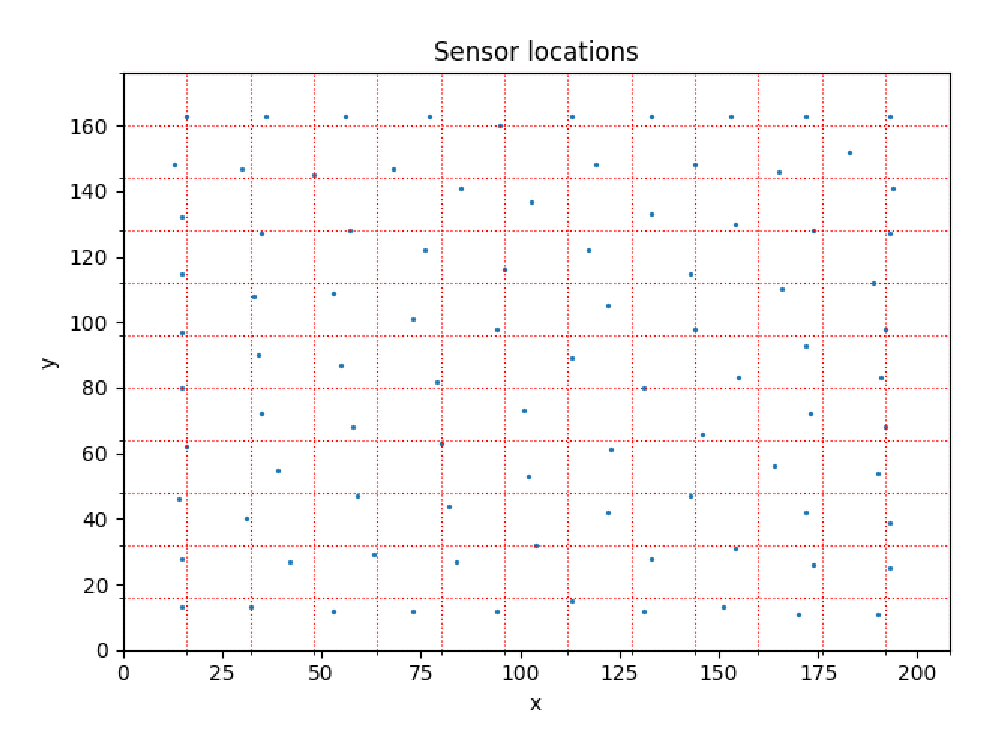
\includegraphics[width=0.45\textwidth]{images/sensors-Nx208-Ny176}
\caption{Example of domain decomposition into ${16{\times}16}$ subdomains. Blue points depict location of sensors pseudo-randomly scattered across the domain. Coordinates are defined as indices of nodal points.}
\label{fig:sensors}
\end{figure}

Since our main objective is to evaluate the capabilities of the Allscale API in real-world applications, the \textit{observation data} will be artificially generated for simplicity. The advantage of having the freedom to generate ``ground-truth'' is that sparsity can be controlled and it can be used to assess the accuracy of the data assimilation solution.  At every time step we extract and record the values of the ground-truth density field $u_{gt}(x,y,t)$ at few sensor locations: $z_s(t)$ = $u_{gt}(x_s,y_s,t)$, $\,\,s \in [1\,{\ldots}\,N_{sensors}]$. The entities $\{z_s(t)\}$ are called \textit{observations} and this is the only information available to the data assimilation method about ``true state of nature''. The sensors themselves are pseudo-randomly scattered across the domain, Figure~\ref{fig:sensors}, where the term ``pseudo-randomly'' means that unrealistic ``clustering'' of sensors is avoided. 

Algorithm~\ref{alg:toplevel} summarizes the major steps in the data assimilation method. The solution propagates forward in time over the period $[0 \ldots T]$ starting from zero density $u(x,y,t)\rvert_{t=0} = 0$. The data assimilation method then nudges towards the actual density as observed by sensors. We employ Kalman filter (line~\ref{alg:line-kalman}) that brings otherwise simulated density closer to observation (if there is a sensor in the subdomain), and this important driving force is responsible for convergence of estimated density field towards the true state. In the absence of observations in a subdomain, the conventional integration step is fulfilled (line~\ref{alg:line-conven}). 

One of the key challenges of the Kalman filter is that it is computationally extremely demanding  \cite{verhaegen1986numerical}, therefore  making it disadvantageous for large scale systems like the one investigated here.
In this work, this issue is resolved by introducing interconnected localised Kalman filters. Specifically, the computational domain of the problem is geometrically decomposed into smaller subdomains. Then the underlying PDE and observation equation are restricted to the introduced subdomains by means of a suitable Domain Decomposition (DD) technique to maintain the continuity of the solutions across the interfaces between the subdomains. These local filters are interconnected by means of DD information exchange mechanisms (they exchange data with each other through boundary conditions). The fully discrete interconnected localised filters are then iterated in order to generate both estimates of the solution of the original PDE.

\begin{algorithm}[!htb]
\caption{Data Assimilation Framework}
\label{alg:toplevel}
\algsetup{indent=2em}
\begin{algorithmic}[1]
\STATE{\small\#\#\# \textit{$*****$ Generator of ground-truth and observations. $*****$}}
\STATE\textbf{Require}: generate ground-truth and observations, Section~\ref{subsec:obsgen}:
{
    \STATE\hspace{2em}{create initial field:} \\
        \STATE\hspace{2em}{$u_{gt}(x,y,t)\rvert_{t=0}$ =
                      $a\,\delta(x-x_c,y-y_c),\,\,\,\forall\,x,y\in\Omega$;}
    \STATE\hspace{2em}{generate a file of pseudo-randomly seeded}
    \STATE\hspace{2em}{sensor locations;}
    \STATE\hspace{2em}{integrate the governing equation (\ref{eq:pde})}
    \STATE\hspace{2em}{forward in time from
                      $t=0\!:\!T$;}
    \STATE\hspace{2em}{while integrating, write a file of observations:}
    \STATE\hspace{2em}{$\{z_s(t)\,|\,s=1\!:\!N_{sensors},\, t=0\!:\!T\}$;}
    \STATE\hspace{2em}{while integrating, store $100$}
    \STATE\hspace{2em}{snapshots of $u_{gt}(x,y,t)$.}
}
\STATE{}
\STATE{\small\#\#\# \textit{$*****$ Data-assimilation solver. $*****$}}
\STATE\textbf{Input}: file of sensor locations, file of observations, 
      initial field $u(x,y,t)\rvert_{t=0} = 0,\,\,\,\forall\,x,y\in\Omega$.
\STATE{\textbf{Require}: sub-divide the whole domain $\Omega$ into a number of subdomains $N_{subdomain}$.}
\STATE{\small\#\#\# \textit{Integrate forward in time and estimate the density field $u(x,y,t)$}.}
\FOR{\label{alg:line-outerloop}\,\,({\small with time-step $\Delta{t}$ (\ref{eq:time-step})})\,\,$t=0$ \TO $T$}
    \FOR{\,\,{\small(\textit{in parallel using Allscale API})}\,\, $c=1$ \TO $N_{subdomain}$}
        \IF{$c$-th subdomain contains at least one sensor}
        \STATE{\label{alg:line-kalman}Solve governing equation (\ref{eq:pde}) forward in time inside $c$-th subdomain using discretization in the form of (\ref{eq:state-propag}): ${\bf u}_{t+1} = {\bf B}^{-1}_t {\bf u}_{t}$.}
        \STATE{Update state inside subdomain using the Kalman filter and previously recorded observations $\{z_s(t)\}$.}
        \ELSE
        \STATE{\label{alg:line-conven}Solve governing equation (\ref{eq:pde}) forward in time inside $c$-th subdomain using discretization in the form of (\ref{eq:state-propag}): ${\bf u}_{t+1} = {\bf B}^{-1}_t {\bf u}_{t}$.}
        \ENDIF
    \ENDFOR
	\STATE{while integrating, store periodic snapshots of $u(x,y,t)$.}
\ENDFOR
\end{algorithmic}
\end{algorithm}

To improve the precision of the data assimilation framework and allow for more accurate specification of sensor location, subdomains are processed at different resolution using the \textit{multi-scaling} capability of Allscale API. Namely, the subdomains with observations are processed at fine resolution because this yields better Kalman filtering estimation. On the other hand, domains without observations (where we just integrate the governing equation) are processed at coarser resolution with less computational cost. 

\subsection{Governing equations}

Advection-diffusion equation is widely used for process modelling in variety of problems. Reader can find many interesting references to the real world applications in \cite{Miyaoka17}.

In this study, we simulate propagation of contaminant in 2D (marine) environment where density is defined as a function of space and time $u$ = $u(x,y,t)$. The physical model of contaminant being dispersed and transported over a spatial domain is described by the following equation:
\begin{equation}
\begin{aligned}
\frac{\partial u}{\partial t} = &
D \left(\frac{\partial^2 u}{\partial x^2} + \frac{\partial^2 u}{\partial y^2}\right)
- v_x \frac{\partial u}{\partial x}
- v_y \frac{\partial u}{\partial y}, 
\\ 
&
\mbox{s.t.}\,\,\,\,\,\,
u\rvert_{t=0} = \delta(x\!-\!x_c,y\!-\!y_c),
\,\,\,\,\,\,u\rvert_{\partial\Omega}=0.
\end{aligned}
\label{eq:pde}
\end{equation}
where $D$ is diffusion coefficient, $v_x = v_x(x,y,t)$, $v_y = v_y(x,y,t)$ are the flow (current) velocity components, the initial condition is defined as point source at some location $(x_c,y_c)$, and the boundary condition is of homogeneous Dirichlet type.

Information external to the computational domain are specified by boundary conditions. Ideally, the absorbing boundary condition should be applied at the outer border $\partial\Omega$ of the domain $\Omega$. In our case, a high density value is mostly obtained far from the boundary and we can go for a simple Dirichlet condition. The paper by Miyaoka (2017) \cite{Miyaoka17}, gives valuable insight into various boundary condition cases pertain to advection-diffusion equation.


\subsection{Domain decomposition}

Allscale API offers two layers of domains discretization. At the top level, the whole domain is represented as a rectangular \textit{grid of subdomains}, and the number of subdomains is not limited in either dimension. Each subdomain is implemented as a \textit{grid of nodal cells}. The size of a subdomain must be fixed because it is defined by template parameters in corresponding \texttt{C++} class and should be available at compile time.

At the run time, each subdomain is assigned to so called \textit{worker} --- either an execution thread or a process in case of distributed application. The assignment and workload balancing is done automatically once the grid of subdomains have been exposed to \textit{parallel for} (\texttt{pfor}) or \texttt{stencil} operator. A portion of subdomain layout is exemplified on Figure~\ref{fig:cell}. As it was already mentioned, computation over each subdomain is conducted independently of other subdomains with no-race-condition guarantee when border points of four immediate neighbour subdomains are being read (green point on Fig.~\ref{fig:cell}). In order to yield a seamless solution we operate over \textit{extended subdomain} that comprises border points of the neighbour subdomains. Extended subdomain is depicted by dotted rectangle on Fig.~\ref{fig:cell}. 

\begin{figure}[!htb]
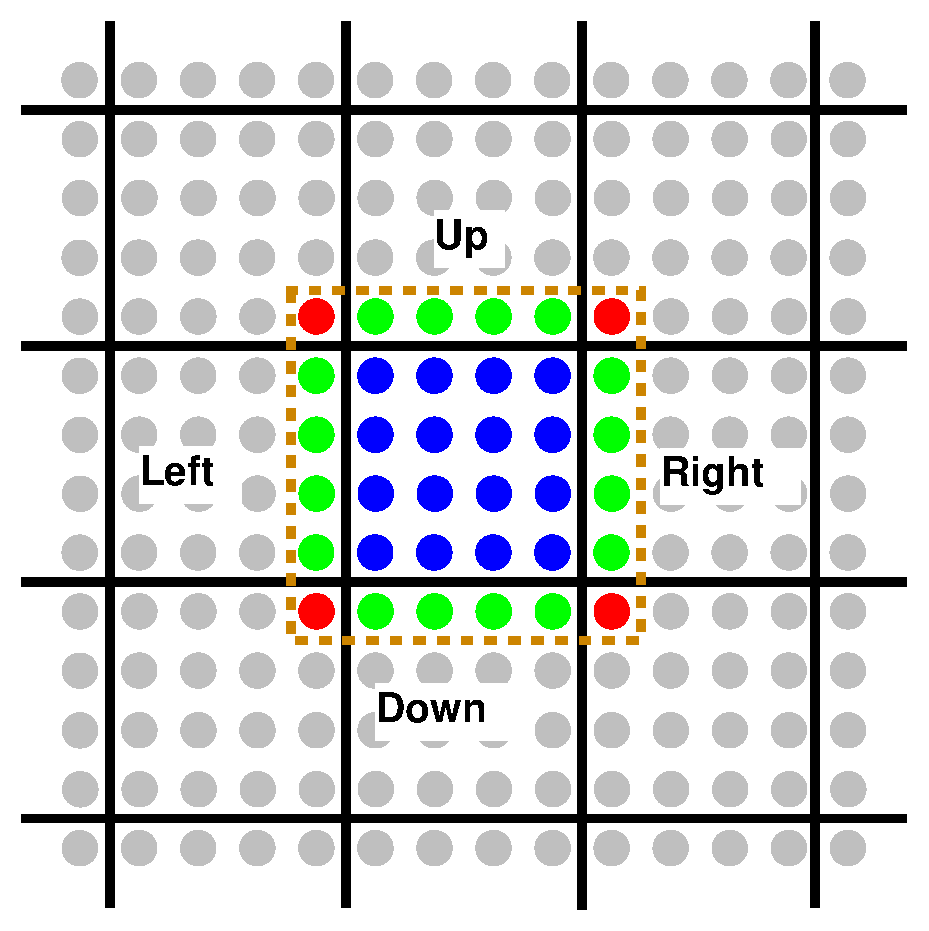
\includegraphics[scale=0.6]{images/subdomain}
\caption{Example of a grid subdomain, constituted by the blue nodal points, and corresponding extended one, outlined by dotted rectangle. Border (green) points of four immediate neighbour subdomains (\textit{Left}, \textit{Right}, \textit{Up}, \textit{Down}) are available for exchange.}
\label{fig:cell}
\end{figure}

\subsection{Finite difference method for state propagation\label{sec:finit-diff}}

Implicit (or backward) Euler method is used in this study for its simplicity, unconditional stability and ability to handle stiff problems, although the method is only first order accurate in time \cite{Sauer11}, \cite{Butcher03}. The second order Crank-Nicolson method is another widely used alternative \cite{Crank47}, \cite{Thomas95}.

%%%%%
\newcommand{\myu}[3]{u_{{#1},{#2}}^{#3}}
%%%%%
Discretization of equation (\ref{eq:pde}) is straightforward: 
\begin{equation}
\begin{aligned}
& \frac{\myu{i}{j}{t+1} - \myu{i}{j}{t}}{\Delta t} = {}\\
& D \left (
\frac{\myu{i+1}{j}{t+1} - 2\myu{i}{j}{t+1} + \myu{i-1}{j}{t+1}}{\Delta{x}^2} +  
\frac{\myu{i}{j+1}{t+1} - 2\myu{i}{j}{t+1} + \myu{i}{j-1}{t+1}}{\Delta{y}^2} \right) \\
& -v_x^{t+1} \frac{\myu{i+1}{j}{t+1} - \myu{i-1}{j}{t+1}}{2\Delta{x}}  
-v_y^{t+1} \frac{\myu{i}{j+1}{t+1} - \myu{i}{j-1}{t+1}}{2\Delta{y}} 
\end{aligned}
\label{eq:discrete-pde}
\end{equation}
where the discrete indices $(i,j)$ run over an extended subdomain, $\Delta{t}$ and $\Delta{x}$, $\Delta{y}$ are the time and space discretization steps respectively.

Flattening 2D arrays $\myu{i}{j}{t}$ and $\myu{i}{j}{t+1}$ into the vectors ${\bf u}_{t}$ and ${\bf u}_{t+1}$ respectively, and collecting other terms into a \textit{sparse} matrix ${\bf B}_t$ the last equation can be rewritten as follows:
\begin{equation}
{\bf u}_{t} = {\bf B}_t {\bf u}_{t+1} \quad \longrightarrow \quad
{\bf u}_{t+1} = {\bf B}^{-1}_t {\bf u}_{t} = {\bf A}_t {\bf u}_{t},
\label{eq:state-propag}
\end{equation}
where ${\bf A}_t = {\bf B}^{-1}_t$ is the \textit{state propagation matrix}. If $(S_x,S_y)$ is the subdomain size and $(S_x\!+\!2,S_y\!+\!2)$ is the size of extended subdomain respectively, then the sparse $((S_x\!+\!2)\!\cdot\!(S_y\!+\!2))\,\,{\times}\,\,((S_x\!+\!2)\!\cdot\!(S_y\!+\!2))$ matrix ${\bf B}$ has $O((S_x\!+\!2)\!\cdot\!(S_y\!+\!2))$ non-zero elements. Considering relatively small subdomain size, the linear system ${\bf u}_{t} = {\bf B}_t {\bf u}_{t+1}$ can solved quite efficiently with respect to unknown ${\bf u}_{t+1}$.

The important trait of the matrix ${\bf B}_t$ is how the extra points of extended subdomain are handled. The operator ${\bf B}_t$ acts according to discretization in (\ref{eq:discrete-pde}) on the regular subdomain points and passes the values at outer points of extended subdomain without change: $\myu{i}{j}{t} = \myu{i}{j}{t+1}$. This mechanism does not affect the finite difference scheme at all, but simplifies software implementation.
%%%%%
\renewcommand{\myu}{}
%%%%%

\subsubsection{Stability}

Although unconditionally stable, the implicit Euler method can develop undesirable artefacts like aliasing and oscillations. We follow practical recommendations suggesting to honour Von Neumann stability criterion derived for \textit{explicit} discretization methods as well as CFL condition. Put together, they give the following upper bound on integration time step:
\begin{equation}
\Delta{t} \le \min\left(
\frac{\min\left(\Delta{x}^2, \Delta{y}^2\right)}{2 D},
\frac{1}{\frac{|v_x|}{\Delta{x}} + \frac{|v_y|}{\Delta{y}}}
\right).
\label{eq:time-step}
\end{equation}

\subsubsection{Flow model}
To simplify things further, we impose the same flow model at each point of the domain $\Omega$. The velocity components are defined as functions of time but not coordinates:
\begin{equation}
\begin{aligned}
& v_x = -v_0 \sin{(0.1 \, t / T - \pi)} \qquad \\
& v_y = -v_0 \sin{(0.2 \, t / T - \pi)}
\end{aligned}
\label{eq:flow}
\end{equation}
where $t$ and $T$ are the current time and integration period respectively, and $v_0$ is a reference velocity supplied by user ($v_0$ = $1\,[m/s]$ by default). 
This readily extends to more complex examples where flow velocities are provided from an external models and thier values are interpolated to the grid using, for example, kriging or any other relevant method.

\subsection{Ground-truth and observations}
\label{subsec:obsgen}
The ground-truth generator integrates discretised equation (\ref{eq:discrete-pde}) forward in time over the entire domain $\Omega$. It takes the same parameters and geometry as the Allscale-based implementation except it does not do any domain decomposition. This forward solver is written in \texttt{Python} programming language for simplicity. Upon completion, two files are generated. The first one contains $100$ snapshots of the entire ``ground-truth'' density field $u_{gt}(x_s,y_s,t)$ (for the accuracy assessment). The seconds file contains observations at sensor locations in format suitable for consumption by the data-assimilation solver. 

As for the initial condition, we set high density value at some internal domain point $(x_c,y_c)$ (contamination point) and zero elsewhere. Note, this is different from case of data-assimilation solver, which starts from zero everywhere density field.

\subsection{Kalman filter}

The Kalman filter produces an estimate of the state of the system as an average of the system's predicted state and of the new measurement using a weighted average. We follow conventional formulation described in many resources, see \cite{Welch06} for example.

Various methods of distributed Kalman filtering have been proposed, but many still suffer from scalability issues or depend on the structure of the problem. A detailed survey of those methods can be found in \cite{mahmoud2013distributed}. The common feature of those methods is that the distribution of filters is done for a discrete model by decomposition of the corresponding matrix, while here, the distribution of filters is done by means of spatial domain decomposition on
a continuous level. Moreover, this work does not depend on the filter formalism,
but applies a decomposition of the problem and observation allowing an independent choice of the local estimators.

\section{Developing parallel DA code within AllScale API}
\label{sec:porting}


The porting to the AllScale API exploits the domain decomposition paradigm of the application to leverage recursive parallelism. Namely, parallelism is implemented by distributing individual subdomains across cores with synchronization and latency hidden to the user. Contrary to a MPI parallel application, where synchronization must be handled by the user via repeated MPI calls, the AllScale implementation has a much closer feel to a serial application. This section presents the main parallel constructs of the AMDADOS application implemented using the library of available AllScale API operators as described in section \ref{sec:API}. These are compared to an equivalent MPI implementation to elucidate on the increased software productivity enabled by the API. In particular, we address the complexity of parallel constructs, explicit synchronization and other concepts considered within the remit of the computer scientist rather than the natural scientist.


\begin{lstlisting}[caption=Sample code to initialize concentrations on all subdomains to zero by means of a parallel loop construct using the pfor operator
, label=initAllSc]
// Initialize the model state variables for all subdomains.
pfor(Point{0,0},  Point{M,N}, [&](const Point_2D & idx) {
    // Iterate through all available grid resolutions.
    for (int layer = LayerFine; layer <= LayerLow; ++layer) {
        state[idx].setActiveLayer(layer);
        // Set all cells within subdomain at that resolution to zero
        state[idx].forAllActiveCells([](double & v) { v = 0.0; });
        // implement knowledge related to external boundary conditions
        ApplyBoundaryCondition(state, idx);
    }
});
\end{lstlisting}


Listing \ref{initAllSc} demonstrates an implementation of a parallel iterator over multiple subdomains within the model. The code segment initialises all subdomain elements to zero. Grid structures are created containing information on the computational structures such as cells, boundary information, position (within global domain), resolution level etc. We initialize this information on an AllScale grid structure (implemented within the AllScale core API at the level of the computer science expert) and loop over a two-dimensional vector \textit{idx} using the \textit{pfor} operator. The idx vector contains information on position of each subdomain from [0,0] to [M,N] where M and N are number of subdomains in x and y respectively. Since the application enables multiple levels of horizontal resolution within each subdomain, initialisation proceeds for all levels. This demonstrates the fundamental concept of the parallel loop construct within the AllScale API. The pfor operator provides a parallel loop execution over a range [0,0] to [M,N] applying a user defined function to each iterator.

\begin{lstlisting}[caption=AllScale Stencil parallel computation, label=stencAllSc]
// solve state solution (state_field) over timestep iterator T
stencil(state_field, T,
  [&](time_t t, const Point & idx, const Grid & state) -> const Grid & {
     // Call numerical solver and data assimilation scheme for each subdomain (idx)
     ComputeSubdomainSolution(configuration, sensors[idx],observations[idx], t,state,grid_variables[idx]);
     // returns model state propagated forward in time and updated with observations (if available)
});
\end{lstlisting}

Parallel DD based solvers are based on the paradigm of distributing the problem across compute cores, solving each state independently and synchronizing solution at intervals (generally each timestep). Listing \ref{stencAllSc} presents the implementation of a space-time decomposition of the problem that provides parallel constructs over the time dimension (T) and the two-dimensional spatial dimension, represented by each subdomain. Within this stencil template, an update operation (in this case a function to compute, or propagate forward, local subdomain solution) is applied to each element of the array. The space-time extents are defined by the \textit{state\_field} (AllScale grid structure containing information on the entire global domain) and the time dimension, \textit{T}. Within this decomposition, a parallel loop over each timestep, \textit{t} and subdomain \textit{state} is conducted. For each update, the user-defined update operation is combining the previous value of the solution within a locally confined area surrounding the targeted subdomain to obtain the updated value. Since each subdomain solution are independent for a single timestep and depend only on direct neighbours for solution synchronization, this provides a valuable resource for parallelism within a space-time decomposition. 


\begin{lstlisting}[caption=AllScale boundary exchange implementation, label=boundAllScale]
// for each subdomain update boundaries in each direction
pfor(Point{0,0},  Point{M,N}, [&](const Point_2D & idx) {
  // init A with current state
  A = state[idx]
  // update boundaries
  for(Direction dir :{Up,Down,Left,Right}){
    // obtain the local boundary
    auto local_boundary = A[idx].getBoundary(dir);
    // obtain the neighboring boundary
    auto remote_boundary =
      (dir == Up)   ? A[idx+{-1,0}].getBoundary(Down ) :
      (dir == Down) ? A[idx+{1,0}].getBoundary(Up    ) :
      (dir == Left) ? A[idx+{0,-1}].getBoundary(Right) :
      (dir ==Right) ? A[idx+{0,1}].getBoundary(Left ) ;
    // compute updated boundary
    assert(local_boundary.size() == remote_boundary.size());
    local_boundary = remote_boundary;
    state.setBoundary(dir,local_boundary);
});
\end{lstlisting}




\begin{figure*}[!h]
\setlength\tabcolsep{0.1em}
\begin{tabular}{ccccc}
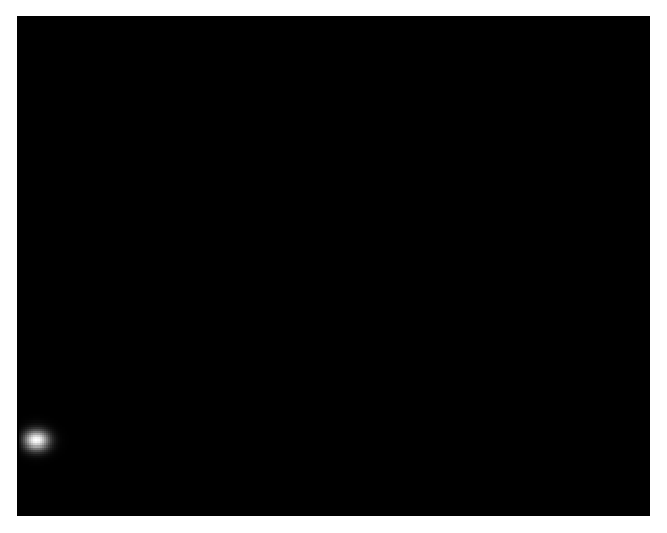
\includegraphics[width=0.19\textwidth]{images/true-field-t=50} &
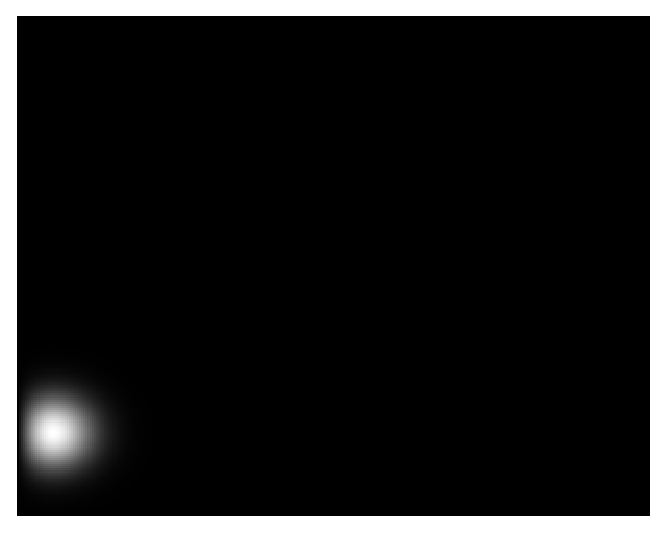
\includegraphics[width=0.19\textwidth]{images/true-field-t=641} &
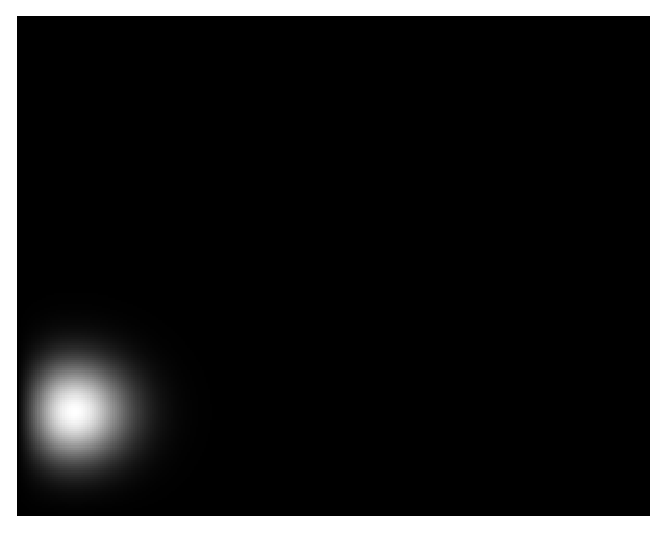
\includegraphics[width=0.19\textwidth]{images/true-field-t=1232} &
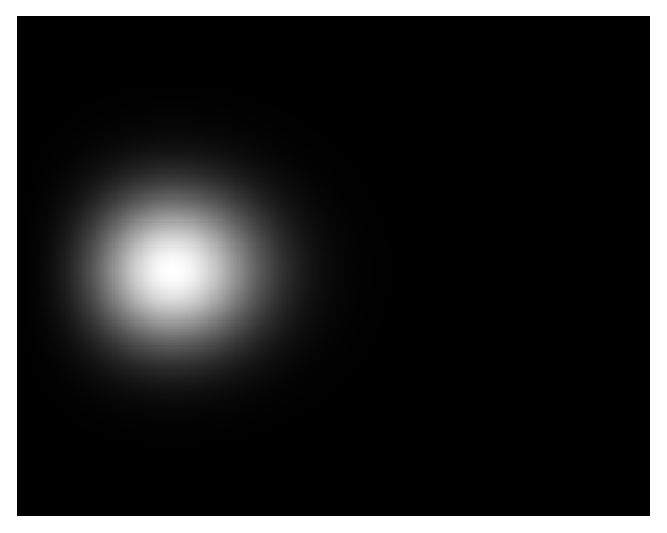
\includegraphics[width=0.19\textwidth]{images/true-field-t=3006} &
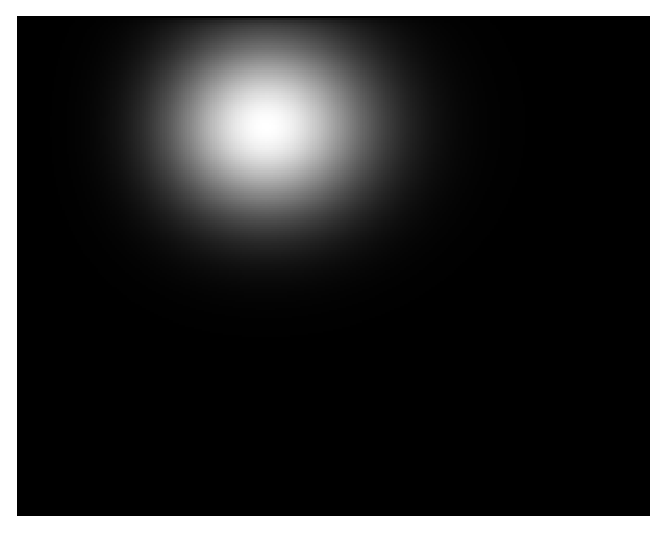
\includegraphics[width=0.19\textwidth]{images/true-field-t=4089} \\
\hline \\
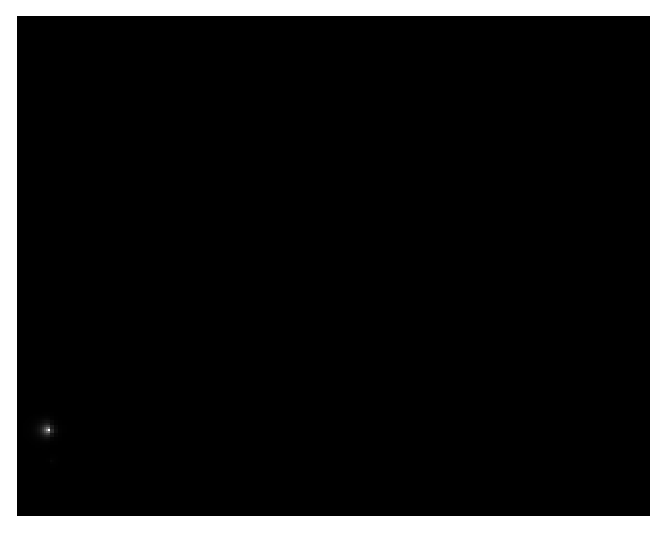
\includegraphics[width=0.19\textwidth]{images/field-t=50} & 
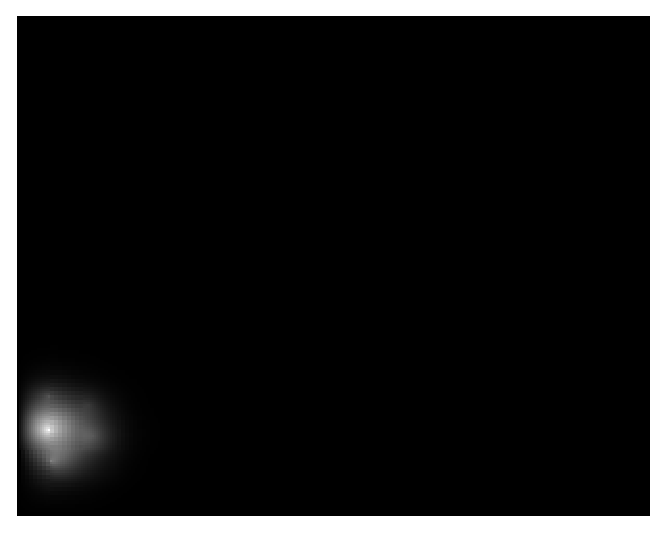
\includegraphics[width=0.19\textwidth]{images/field-t=641} &
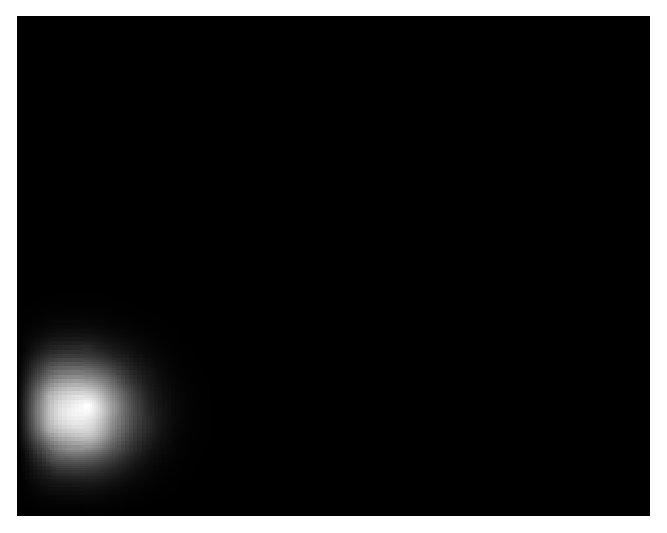
\includegraphics[width=0.19\textwidth]{images/field-t=1232} & 
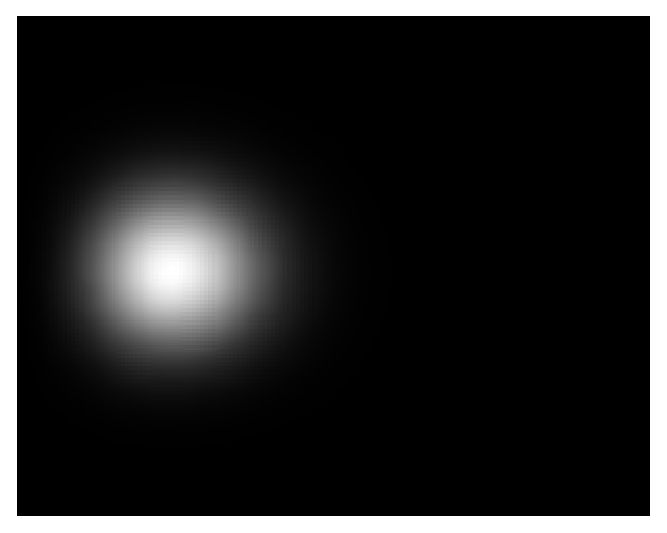
\includegraphics[width=0.19\textwidth]{images/field-t=3006} &
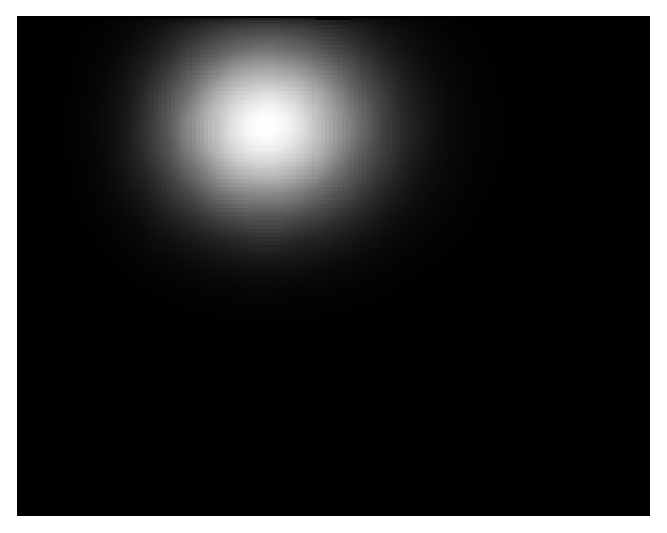
\includegraphics[width=0.19\textwidth]{images/field-t=4089} 
\end{tabular}
\caption{Simulation of advection-diffusion process. \textit{Top row}: Evolution in time of the ``correct'' solution computed offline as a single global domain. \textit{Bottom row}: data-assimilation solution that starts from zero density field and gradually catches up the ground-truth. There are $72960$ nodal points representing $304{\times}240$ domain and $182$ sensors pseudo-randomly scattered therein.}
\label{fig:density}
\end{figure*}




Exchange of boundary information to maintain solution fidelity is central to DD approaches. Within the AllScale API, synchronisation aspects are managed at the core API level facilitating trivial implementation of boundary exchange operations. Listing \ref{boundAllScale} outlines how we code boundary exchanges. Neighbouring domains (if they exist) are identified via Boolean data types. On each of the four boundaries, the overlapping local boundary are replaced by the computed values from the neighbouring, remote boundary. All additional synchronization considerations such as send/receive orderings, computational overlapping, etc. are managed at the level of the core API, hidden from the application developer. Further, despite the stencil implementation providing a complete space-time decomposition, the API ensures that data from the appropriate time level are communicated. 


As a comparison, Listing \ref{boundMPI} presents a section of code demonstrating how boundary exchange in an MPI implementation of the code may look. Within this paradigm, the application loops over each boundary (where neighbour domain exists), packs boundary data and sends to its neighbour via an MPI\_Send communication. The neighbouring domain must receive the data  via a  corresponding MPI\_Recv call. Further care must be taken in the order of MPI\_Send/MPI\_Recv calls to avoid blocking by a process awaiting communication. The simplified coding structure of the AllScale API removes many of these manual synchronization requirements greatly reducing coding complexity.

Apparent is the greatly simplified coding implementations enabled by the AllScale API. Applying operations to all elements is similar to a serial application with a parallel for (\textit{pfor}) operator substituting the classical for operator. Other common parallel operations such as data exchange between separate grids are also greatly simplified. By following the templates provided by the AllScale SDK it is evident that users can develop a huge range of domain decomposition based applications with little knowledge of HPC or parallel computing concepts (i.e. simply by learning AllScale specific development skills). 

\begin{lstlisting}[caption= Sample MPI implementation of boundary exchange and synchronization within a DD problem
, label=boundMPI]
// For each subdomain, loop over boundaries and check
// whether boundaries exist in each direction and synchronise
for (size_t ind = 0; ind < 4; ind++)  
{   
    Connection * conn = decProb->connections[ind];  
    // for each subdomain boundary check if neighbour exist to East or West  
    if (conn->lhs == subProblem || conn->rhs == subProblem)  
    {
        // get connection nodes index and subproblem
        if (conn->rhs == subProblem)     //  neighbour to the West
        {
            PackSendMPI(decProb, subProblem, conn, timestep, bcType, -1, proc_id);
        }
        if (conn->lhs == subProblem)     // neighbour to the East 
        {
            // Receive boundary data from East 
            RecvUnpackMPI(decProb, subProblem, conn, timestep, bcType, -1, proc_id);
            // Send boundary data to East
            PackSendMPI(decProb, subProblem, conn, timestep, bcType, -1, proc_id);
        }
        if (conn->rhs == subProblem)     // neighbour to the West
        {
            // Receive boundary data from West 
            RecvUnpackMPI(decProb, subProblem, conn, timestep, bcType, -1, proc_id);
        }
    } 
    if (conn->up == subProblem || conn->down == subProblem)  
    {
        ...  // For neighbour subdomains to the South and North
        ...  // repeat equivalent exchange of boundary data 
        ...  // and synchronisation as implemented for East and West above
    }     
}
\end{lstlisting}







\section{Results and Discussion}

Domain decomposition based approaches have huge applicability in simulation due to the promise of reduced computational demand (by distributing across compute resources, reducing the size of linear algebra matrices, etc.). An important consideration however, is to ensure fidelity of the solution; i.e. the computed solution should be qualitatively (if not quantitatively) equivalent to that computed if modelled as a single global domain. This is particularly important for implementations such as the AllScale API where many parallel constructs are managed at the kernel level, outside the remit of the application developer. Further, the space-time decomposition raises the possibility that data communication may be contaminated by transfer from incorrect timesteps. Implementations using a novel technology such as AllScale, at a relatively low level of maturity, requires careful analysis of results to ensure fidelity. The current implementation provides a valuable benchmark of correctness as the observation generator used to provide data for the assimilation scheme also serves as the true solution. Hence, computed results can be readily compared against these data. Figure~\ref{fig:density} presents snapshots of results from a number of stages during the simulation cycle. Results are compared to the ``correct'' solution computed as part of the observation generator routine (i.e. routine that generates data for assimilation into the model).



Figure~\ref{fig:relerr} shows how relative error fades away as simulation progresses. The relative error is computed as a ratio between $L_2$-norm of field of density difference and  $L_2$-norm of ground-truth density: $\varepsilon$ = $\|u_{gt} - u\|_2/\|u_{gt}\|_2$. The data-assimilation solver behaves as expected in nudging the solution towards the correct solution. It catches up the true distribution as soon as the first sensor has been touched by a high-density spot. Of importance, no contamination of results develops from boundary exchange protocols; i.e.  no aliasing is evident at subdomain boundaries in Figure~\ref{fig:density} while Figure~\ref{fig:relerr} demonstrates that data assimilation directs error towards zero over time. 

\begin{figure}
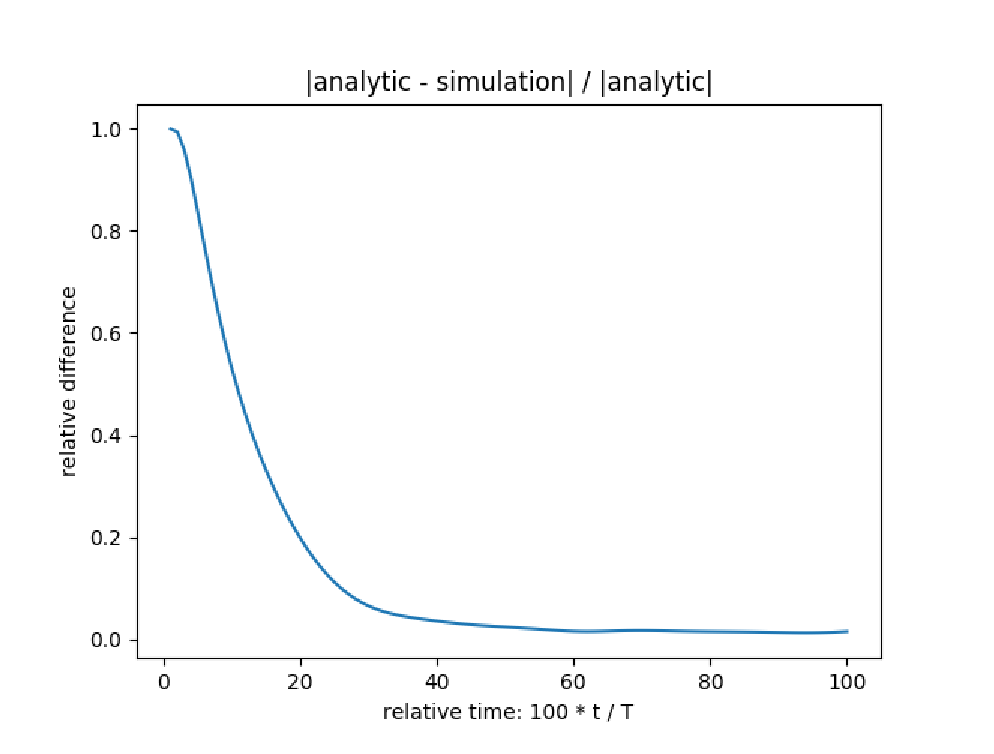
\includegraphics[scale=0.5]{images/rel-diff-Nx304-Ny240}
\caption{Relative difference ($\varepsilon$ = $\|u_{gt} - u\|_2 / \|u_{gt}\|_2$) between the ground-truth density and data-assimilation solution, as a function of ``relative time'': $\tau$ = $100\,t / T$, where $t$ is a physical time in seconds, and $T$ is an integration period.}
\label{fig:relerr}
\end{figure}

 Performance results are a key metric of this analysis. Experiments focus on shared memory parallelism to provide insights into throughput, contention and parallel performance at different levels of load allocation. Tests were conducted on compute server with 2 Intel Xeon 2.20GHz processors providing total of 44-core machine with Linux RedHat-7.4, 64-bit operating system.  The first test investigates strong scaling performance to gain insight into both algorithmic and AllScale scalability. A key consideration of all tests was how the application scales within the grid-based implementation, i.e. to understand what the relative proportions of computation, communication and management of the compute workloads and distribution are. Figure \ref{fig:scalability} presents the strong scaling results. The problem size is fixed and the number of working threads increased from 1 to 44 in a series of simulations.  In general results exhibit acceptable performance. Increasing the number of CPU cores significantly reduces the simulation time before plateauing as parallel overheads saturate.  

\begin{figure}
\begin{tabular}{cc}
\includegraphics[width=0.48\textwidth]{images/ScalabilitySize_redo} \\
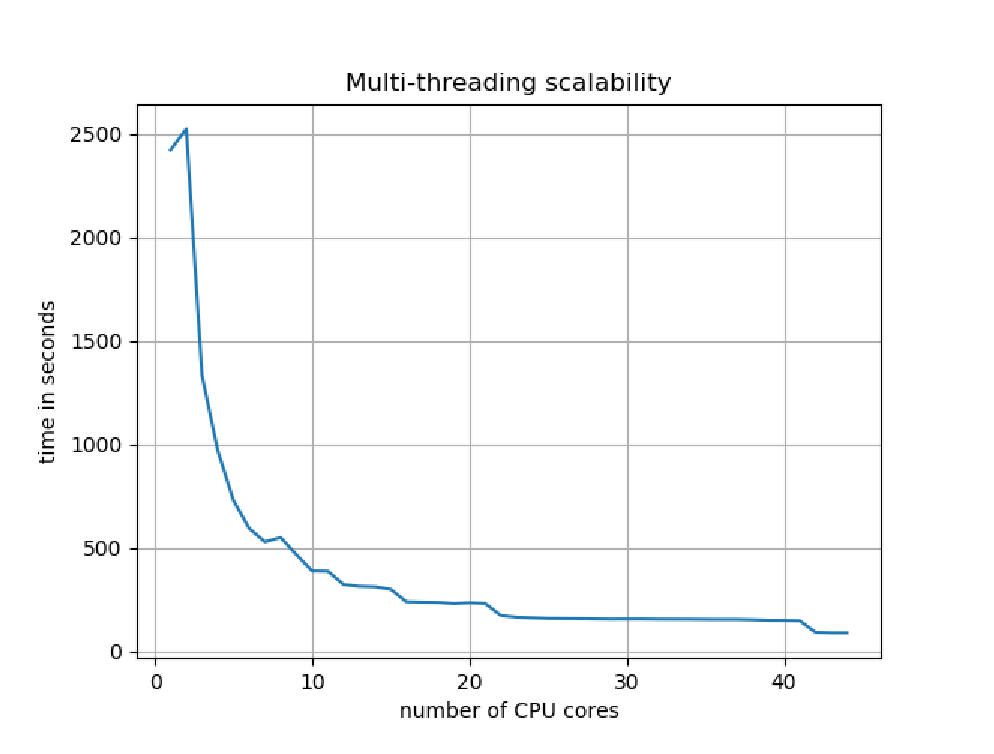
\includegraphics[width=0.48\textwidth]{images/scalability-mt} 
\end{tabular}
\caption{Scalability test results using the AllScale API. size scalability (top): execution time vs. problem size with all compute resources available. Multi-threading scalability (bottom): execution time plotted against the number of working threads.}
\label{fig:scalability}
\end{figure}

The second test investigates the total computational throughput of the application. We enabled all the CPU resources to the application increasing the problem size (number of subdomains) in a series of simulations. Figure \ref{fig:scalability} presents results of this experimental study. For this experiment ideal scaling would be a linear increase in simulation time as the problem size is increased; this trend is largely respected with simulation time increasing approximately as linear function of problem size. 

A key result of this study that is more difficult to quantify is developer productivity. Even for a relatively small HPC study, ease of programming is greatly improved. At the simplest level, aspects related to synchronisation and message passing are removed from the developer's responsibility. Moving to a higher level of abstraction, aspects related to the hardware architecture are managed at the core API level, meaning that the domain expert is not exposed to complex topics related to the tuning of the application for various architectures: these are handled by the computer scientist at the data structure level, again removed from any domain specific algorithmic implementations. Finally, since data structures are self-contained representations of each subdomain solution at the core API level, aspects related to load balancing are removed from the developer's view, eliminating complex and code-intensive aspects such as overlapping computation and communication and other cumbersome load balancing approaches. Instead, load balancing can be managed at higher level of abstraction using advanced online monitoring and management complex. We estimate that developer productivity is increased by at least 50\% by the AllScale user API compared to traditional approaches such as MPI. 


\section{Conclusion}
This study demonstrates the capabilities of the AllScale API implementation and its feasibility as part of the next generation of HPC programming environments. Developing within the AllScale user API provides many advantages to the scientist. User productivity is greatly enhanced as parallel structures are hidden at the core level of the API. This advantage is particularly true for users writing new parallel code from scratch as one simply follows the provided template and write the code in a manner very similar to serial code. All programming is done in pure C++ eliminating the need to learn any specific parallel tools. 

The application is currently limited to shared memory parallelism and we aim to release a distributed memory parallel version in June 2018. In particular, large scale experiments will be conducted to evaluate 1) scalability of the code at the many 1000 core level, 2) performance of load balancing (data assimilation provides a valuable test-case due to the very different computational expense of subdomains depending on whether observation exists or not) and 3) detailed evaluation of the performance of the recursive parallel space-time decomposition

%% Bibliography
\bibliographystyle{IEEEtran}
\bibliography{masterbib}
%\bibliography{references}



% trigger a \newpage just before the given reference
% number - used to balance the columns on the last page
% adjust value as needed - may need to be readjusted if
% the document is modified later
%\IEEEtriggeratref{8}
% The "triggered" command can be changed if desired:
%\IEEEtriggercmd{\enlargethispage{-5in}}

% references section

% can use a bibliography generated by BibTeX as a .bbl file
% BibTeX documentation can be easily obtained at:
% http://mirror.ctan.org/biblio/bibtex/contrib/doc/
% The IEEEtran BibTeX style support page is at:
% http://www.michaelshell.org/tex/ieeetran/bibtex/
%\bibliographystyle{IEEEtran}
% argument is your BibTeX string definitions and bibliography database(s)
%\bibliography{IEEEabrv,../bib/paper}
%
% <OR> manually copy in the resultant .bbl file
% set second argument of \begin to the number of references
% (used to reserve space for the reference number labels box)


% that's all folks
\end{document}


